\ctitle{Likevekt mellom væske, faste stoffer og gasser}
\paragraph{Dette kapittelet}
Kjemisk potensial beskriver også partiklenes tendens til å bevege seg mellom to faser, for eksempel mellom en væskefase og en fast fase.

\cstitle{Hvorfor fordamper væsker?}
\label{sec:vaporcompetingdrivingforces}
Vi behandler damp som en ideell gass. Da er det temperatur og trykk som avgjør hvor mye vi får av gass og væske gjennom en balanse mellom to konkurrerende drivkrefter: 
\begin{enumerate}
	\item Attraktive intermolekylære krefter holder molekylene sammen i væskefasen.
	\item Entropien til partiklene (eller mer presist: trans\-lasjonskomponenten til entropien) øker når de går over i gassfasen.
\end{enumerate}
Vi kan se på ligningene for endring i Gibbs' og Helmholz' fri energi for å se hvorfor økt temperatur fører til at væsker fordamper:
\begin{align}
	\Delta G &= \Delta H - T\Delta S \\
	\Delta F &= \Delta U - T\Delta S
\end{align}
$\Delta H$- og $\Delta U$- leddene representerer her energien som må til for å bryte de attraktive intermolekylære bindingene, mens $T\Delta S$-leddet representerer entropiøkningen ved å gå over i gassfasen.

\cstitle{Damptrykk}
\paragraph{Likevekt mellom gass og væskefase.} Vi kan regne gass-væske-likevekter med nøyaktig samme prosedyre som for kjemiske likevekter. Vi ser på $N_L$ partikler i væskefase og $N_G$ partikler i dampfase. Hvis vi holder $(p,T,N)$ konstant (slik at det er Gibbs fri energi som skal minimeres) får vi ligningen
\begin{equation}
	dG=\mu_GdN_G+\mu_LdN_L
\end{equation}
der 
\begin{equation}
	dN = dN_G + dN_L = 0
\end{equation}
slik at
\begin{equation}
	dG=(\mu_G-\mu_L)dN_L
\end{equation}
ved likevekt er $dG=0$ slik at
\begin{equation}
	\label{vaporliquidequilibrium}
	\mu_G = \mu_L
\end{equation}
Så husker vi tilbake til \eqref{idealgaschemicalpotential} at, for en ideell gass, er
\begin{equation}
	\mu_G = k_BT\ln\frac{p}{p_{\text{int}}^o}.
\end{equation}

\paragraph{Det kjemiske potensialet til den konsenserte fasen} Vi har altså $\mu_G$, men vi trenger fortsatt en modell for $\mu_L$ for å kunne forutsi egenskapene til gass-væske-likevekten. Vi begynner med en gittermodell der vi \emph{ser bort i fra forskjellen mellom væske og fast stoff}, og kaller begge deler for en \i{kondensert fase}. Dette er i utgangspunktet OK fordi væsker er 1000 ganger tettere enn gasser, mens fast stoff sjelden er mer enn 10\% tettere enn væske. En slik modell gjør også en tilnærmelse ved å se bort i fra at væsker ikke har den samme regulariteten og periodisiteten som fast stoff. Antallet nærmeste naboer varierer også i en væske, men \emph{gjennomsnittet} av antallet nærmeste naboer er heldigvis ganske veldefinert.

Siden væsker og faste stoffer er mye mindre kompressible enn gasser (volumet forandrer seg lite når trykket er konstant), er det ikke så nøye om vi velger konstant trykk $(T,p,N)$ eller konstant volum $(T,V,N)$. Vi kan derfor velge om vi vil minimere henholdsvis $G$ eller $F$. Siden det i mikroskopiske modeller ofte er enklere å bruke konstant $V$ enn konstant $p$, velger vi å minimere $F=U-TS$.

Vi begrenser oss til å se på interaksjoner mellom nærmeste naboer. Hvis to partikler av type $A$ er bundet til hverandre (ved å være på tilstøtende plasser i gitteret) har de en attraktiv bindingsenergi 
\begin{equation}
	w_{AA}<0
\end{equation}
seg imellom. Vi ser på denne som uavhengig av temperatur - dette er en god tilnærmelse for kovalente bindinger, så dermed har vi i det minste en god modell for faste stoffer. Multiplisiteten til bindingen er 1, siden det ikke betyr noe hvis partiklene bytter plass. Dermed er entropien assosiert med bindingen lik $S=k_B\ln W = 0$. Vi ignorerer også bidrag fra vibrasjon og rotasjon i væsken.

Hver partikkel har $z$ nærmeste naboer (\i{koordinasjonstallet} er $z$). Hver binding er delt mellom to partikler, så vi assosierer en energi $\frac{1}{2}zw_{AA}$ med hver partikkel. Dermed blir den totale indre energien 
\begin{equation}
	\label{bondingenergy}
	U = \frac{1}{2}Nzw_{AA}
\end{equation}
og den frie energien blir
\begin{equation}
	F = U - TS = U - 0 = \frac{1}{2}Nzw_{AA}
\end{equation}
og det kjemiske potensialet blir
\begin{equation}
	\mu_L = \left(\frac{\partial F}{\partial N}\right)_{T,V} = \frac{1}{2}zw_{AA}
\end{equation}

\paragraph{Damptrykk} Nå kan vi erstatte hver side av $\mu_G=\mu_L$ med de respektive uttrykkene for $\mu_G$ og $\mu_L$. Vi har at
\begin{equation}
	k_BT\ln\frac{p}{p_{\text{int}}^o}=\frac{1}{2}zw_{AA}
\end{equation}
Dette kan vi løse for å finne trykket ved likevekt. Dette trykket, som kalles \i{damptrykket}, er
\begin{equation}
	\label{vaporpressure}
	p=p_{\text{int}}^oe^{\frac{zw_{AA}}{2k_BT}}.
\end{equation}
Merk at dette trykket også er proporsjonalt med \emph{tettheten av partikler i gassfase}, på grunn av den ideelle gassloven: $p = (N/V)k_BT$. Et høyt damptrykk betyr altså at molekyler foretrekker å befinne seg i gassfase, mens et lavt damptrykk betyr at molekylene heller vil være i en kondensert fase. Det er denne tolkningen som gir den beste forståelsen av hva som skjer når damptrykket dukker opp senere.

Modellen vår forutsier to ting:
\begin{itemize}
	\item Hvis bindingene mellom partiklene blir sterkere, synker damptrykket (fordi $w_{AA} < 0$).
	\item Hvis temperaturen øker, øker også damptrykket.
\end{itemize}
Dette stemmer overens med det vi påsto i begynnelsen av forrige delkapittel.

\cstitle{Hulrom i væsker og faste stoffer}
For å fjerne en partikkel fra gitteret må man bryte $z$ bindinger, som koster den den positive energien $\Delta U_r=-zw_{AA}$. Denne energien er assosiert med ``løse bindinger'', så halvparten av energien ender opp i partikkelen, og halvparten fordeles blant partiklene rundt hulrommet. Dette er fordi man bryter de $z/2$ som tilhører den forsvinnende partikkelen, og de $z/2$ bindingene som tilhører de andre partiklene rundt. Vi antar her at hulrommet ikke forvrenges eller justerer seg etter at partikkelen har forsvunnet (i så fall vil energien synke litt).

Hvis man fjerner en partikkel og så lar gitteret tilpasse seg endringen ved å lukke hulrommet, vil dette innebære en energiforskjell $\Delta U_{r,\ c}$ som er lik forskjellen i energi mellom et system med $N-1$ partikler og et system med $N$ partikler: 
\begin{equation}
\Delta U_{r,\ c}=U(N-1)-U(N)=-\frac{zw_{AA}}{2}.
\end{equation}
Da blir energien assosiert med å lukke et hulrom $\Delta U_c = \frac{zw_{AA}}{2}$ og energien assosiert med å åpne et hulrom $\Delta U_o=-\frac{zw_{AA}}{2}$.

\cstitle{Trykk som funksjon av temperatur ved faselikevekt: Clapeyrons ligning}
Denne seksjonen inneholder den mer tradisjonelle termodynamiske behandlingen av faselikevekt. Et typisk fasediagram er et $(p,T)$-diagram med $T$ på den horisontale aksen og $p$ på den vertikale aksen. Likevekten mellom to faser tegnes inn som en kurve, som i Figur \ref{fig:fasediagram}. La oss finne et uttrykk for stigningstallet til denne kurven.

\begin{figure}[H]
	\centering
	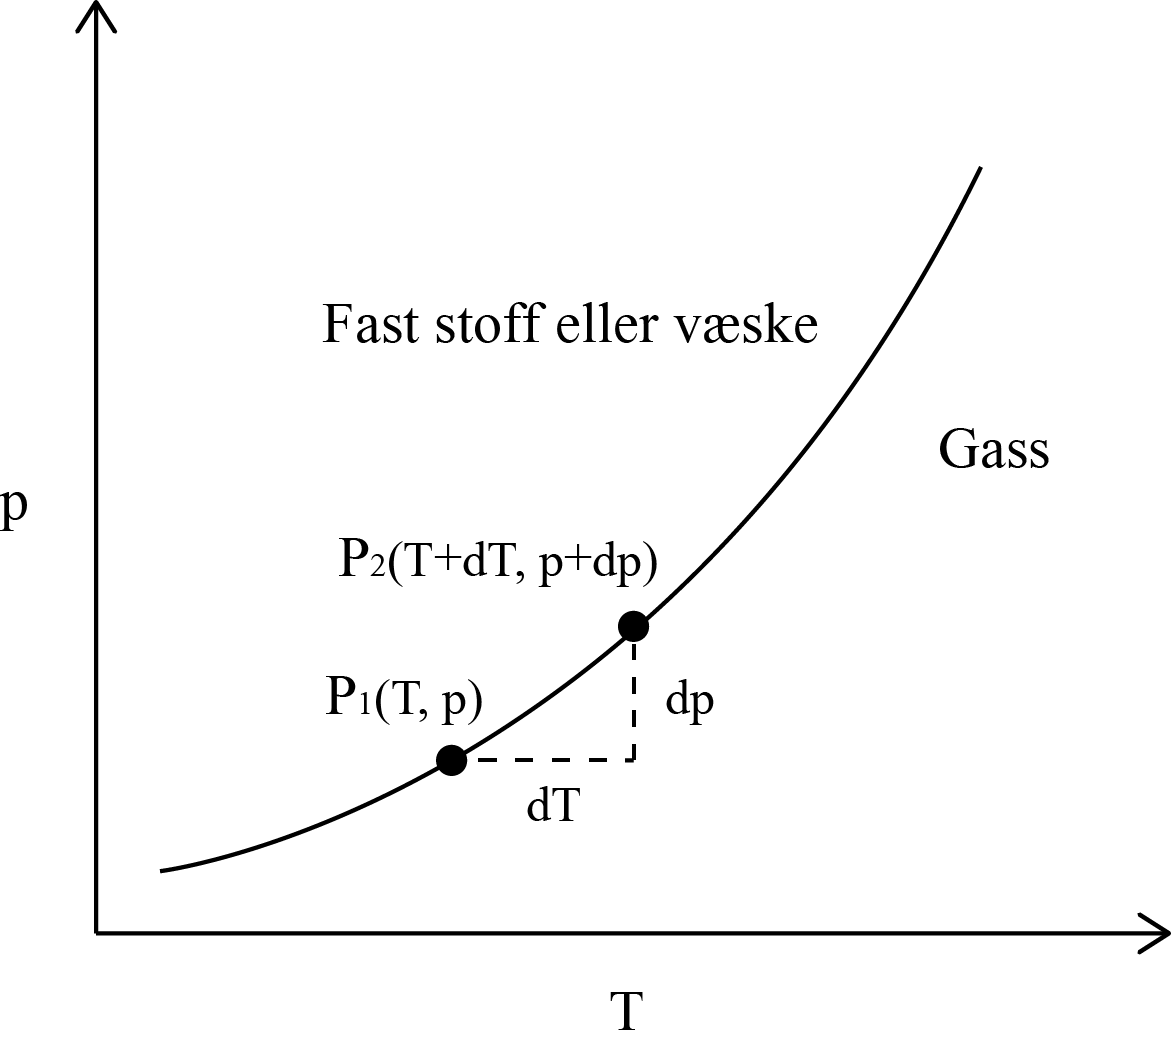
\includegraphics[width=0.35\textwidth]{eigenfig/phase.png}
	\caption{et fasediagram!}
	\label{fig:fasediagram}
\end{figure}

Vi ser på to punkter, svært nær hverandre, begge på likevektskurven,
\begin{align}
    P_1 &= (T,p) \\ P_2 &= (T+\dT,p+\dpp),
\end{align}
der \eqref{vaporliquidequilibrium} gir at 
\begin{align}
	\mu_L(T,p)&=\mu_G(T,p) \\ \mu_L(T+\dT,p+\dpp)&=\mu_G(T+\dT,p+\dpp).    
\end{align}
Det kjemiske potensialet ved $(T+\dT,p+\dpp)$ er resultatet av en liten forandring i potensialet ved $(T,p)$, så
\begin{equation}
	\mu_L(T+\dT,p+\dpp) = \mu_L(T,p) + \text{d}\mu_L
\end{equation}
\begin{equation}
	\mu_G(T+\dT,p+\dpp) = \mu_G(T,p) + \text{d}\mu_G
\end{equation}
Hvis vi kombinerer de fire forrige ligningene, får vi at
\begin{align}
    \mu_L(T+\dT,p+\dpp)&=\mu_L(T,p)+\text{d}\mu_L \\
    \mu_L(T+\dT,p+\dpp)&=\mu_L(T,p)+\text{d}\mu_G,
\end{align}
og endelig
\begin{equation}
	\label{dmugdmul}
	\text{d}\mu_G=\text{d}\mu_L.
\end{equation}
siden vi ser på $\mu$ som en funksjon av $T$ og $p$ har vi at
\begin{equation}
	\label{dmu}
	\text{d}\mu=\left(\frac{\partial \mu}{\partial T}\right)_{p,N}\dT+\left(\frac{\partial \mu}{\partial p}\right)_{T,N}\dpp
\end{equation}
Når vi bruker frie energier \emph{per mol} som enhet for $\mu$, vet vi at de partiellderiverte i \eqref{dmu} er molar entropi $s$ og molart volum $v$ gjennom følgende Maxwellrelasjoner:
\begin{equation}
	\left(\frac{\partial \mu}{\partial T}\right)_{p,N}=-\left(\frac{\partial S}{\partial N}\right)_{T,p} = -s
\end{equation}
\begin{equation}
	\left(\frac{\partial \mu}{\partial p}\right)_{T,N}=\left(\frac{\partial V}{\partial N}\right)_{T,p} = v
\end{equation}
så kombinasjonen av \eqref{dmugdmul} og \eqref{dmu}, innsatt ligningene over, blir
\begin{equation}
	-s_G\dT+v_G\dpp=-s_L\dT+v_L\dpp
\end{equation}
som vi stokker om på for å få at
\begin{equation}
	\label{soonclapeyron}
	\frac{\dpp}{\dT} = \frac{s_G-s_L}{v_G-v_L} = \frac{\Delta s}{\Delta v}
\end{equation}
Ved faseovergangen er endringen i den molare frie energien $\Delta \mu=0$, og siden $\Delta \mu = \Delta h - T\Delta s = 0$, får vi at
\begin{equation}
	\Delta s = \frac{\Delta h}{T}
\end{equation}
Dette settes inn i \eqref{soonclapeyron} for å få \i{Clapeyrons ligning}:
\begin{equation}
	\label{clapeyron}
	\frac{\dpp}{\dT} = \frac{\Delta h}{T\Delta v}
\end{equation}
Det molare volumet til gassfasen er mye større enn det molare volumet til den konsenserte fasen. Hvis vi kombinerer dette med den ideelle gassloven, får vi at
\begin{equation}
	\Delta v = v_G-v_L \approx v_G = \frac{RT}{p}
\end{equation}
Vi bruker $R=N_Ak_B$ i ligningen fordi vi her snakker om volum per mol. Dette gir oss at
\begin{equation}
	\frac{1}{p}\frac{dp}{dT}=\frac{\Delta h}{RT^2}
\end{equation}
Når vi setter inn at $\frac{\text{d}\ln p}{\dT}=\frac{1}{p}\frac{\dpp}{\dT}$, får vi \i{Clausius-Clapeyron-ligningen}
\begin{equation}
	\label{clausiusclapeyron}
	\frac{\text{d}\ln p}{\dT}=\frac{\Delta h}{RT^2}
\end{equation}
Når $\Delta h$ er uavhengig av $p$ pg $T$ kan vi integrere opp ligningen for å få at
\begin{align}
	\int_{p_1}^{p_2}\text{d}\ln p&=\int_{T_1}^{T_2}\frac{\Delta h}{RT^2}\dT \\ \ln\frac{p_2}{p_1}&=-\frac{\Delta h}{R}\left(\frac{1}{T_2}-\frac{1}{T_1}\right),
\end{align}
så $\ln p$ avhenger lineært av $1/T$. Verdien for $\Delta h$ får vi gjerne fra tabeller. Med denne ligningen kan vi forutsi et kokepunkt $(p_2,T_2)$ dersom vi kjenner et annet kokepunkt $(p_1,T_2)$.

La oss se litt nærmere på \eqref{soonclapeyron}: $\frac{dp}{dT} = \frac{\Delta s}{\Delta v}$. Dersom stigningstallet $\frac{dp}{dT}$ til faselikevekten er positivt, vil fasen med størst entropi også ha størst volum. Dette er tilfellet for alle faseoverganger mellom væske og gass og mellom fast stoff og gass. Det er også som regel tilfellet for faseovergangen mellom væske og fast stoffm men et viktig unntak her er vann. For vann er $\frac{dp}{dT}<0$, og siden vann i væskeform har høyere entropi enn is, forutsier \eqref{soonclapeyron} noe vi allerede vet: at vann i væskeform har et mindre molart volum enn is.

\cstitle{Kjøleskap og varmepumper}
Kjøleskap og varmepumper absorberer varme fra et kaldt sted og slipper det ut på et varmere sted. Dette skjer ved at et fluid pumpes gjennom et rørsystem og gjennomgår en termodynamisk syklus av fordampning og kondensasjon. Disse maskinene benytter seg av to ting:
\begin{itemize}
	\item Fordamping lagrer energi ved å bryte ikke-kovalente bindinger, og kondensasjon gir denne energien tilbake.
	\item En væske kan fordampes ved lav temperatur og senere kondenseres ved høy temperatur ved å kontrollere trykket.
\end{itemize}
Se s. 264-265 for en gjennomgang av hvert trinn i den termodynamiske syklusen.

\cstitle{Overflatespenning: likevekt mellom overflate og bulk}
En \i{overflate} defineres som grensen mellom en kondensert fase og en gassfase. Dette er et spesialtilfelle av en \i{grenseflate}, som er grensen mellom to vilkårlige faser. \i{Overflatespenning}en $\gamma$ er den frie energien det koster oss å øke overflatearealet til et system. Som vi så i kapittel 9 kan de fundamentale ligningene våre utvides til å ta hensyn til en slik overflatespenning: $\dFh'=\dFh+\gamma\dA$. 

\paragraph{En gittermodell for overflatespenning} Vi ser for oss et materiale i kondensert fase som består av $N$ identiske molekyler. Av disse er $n$ molekyler på overflaten, mens de resterende $N-n$ er ``bulk''. Bulkmolekylene har $z$ nærmeste naboer, mens overflatemolekylene har $z-1$ nærmeste naboer (siden de er eksponert på overflaten). Hvis vi husker tilbake til \eqref{bondingenergy}, blir den totale indre energien som er lagret i bindinger:
\begin{equation}
	\label{surfacetensiontotalenergy}
	U=\frac{1}{2}zw_{AA}(N-n)+\frac{1}{2}(z-1)w_{AA}n=\frac{1}{2}w_{AA}(Nz-n)
\end{equation}
Multiplisiteten er $W=1$ fordi alle molekylene er identiske, slik at materialets tilstand er identisk uansett hvor mange molekyler som bytter plass. Derfor er $S=0$ og $F=U$. Så har vi at 
\begin{equation}
	\gamma = \left(\frac{\partial F}{\partial A}\right)_{T,V,N} = \left(\frac{\partial F}{\partial n}\right)_{T,V,N}\frac{\dn}{\dA} = \left(\frac{\partial U}{\partial n}\right)_{T,V,N}\frac{\dn}{\dA}
\end{equation}
Arealet er $A=na$, der $a$ er arealet per partikkel. Så $n=\frac{A}{a}$ og $\frac{\dn}{\dA}=\frac{1}{a}$. Fra \eqref{surfacetensiontotalenergy} får vi at $\left(\frac{\partial U}{\partial n}\right)_{T,V,N}=-w_{AA}/2$. Dermed er overflatespenningen:
\begin{equation}
	\gamma = -w_{AA}/2a
\end{equation}
$\gamma$ har følgende egenskaper:
\begin{itemize}
	\item $\gamma$ er positiv, siden $w_{AA}<0$.
	\item $\gamma$ er den frie energien det koster å bevege et molekyl fra bulk til overflaten, slik at arealet øker med $\dA$.
\end{itemize}
Hvis det er sterke intermolekylære krefter i materialet, er $\gamma$ stor. En stor overflattespenning gjør at materialet trekker seg sammen til den har en form med minimalt overflateareal. Dette er forklaringen på at vann danner kulerunde dråper i verdensrommet: en kule er formen som har minst areal per volum.
